\documentclass[11pt]{article}
\usepackage[textwidth=18.0cm, textheight=23.0cm, top=2.0cm]{geometry}
\usepackage{pst-all}
\usepackage{amssymb}
\usepackage{tikz}
\usepackage{underscore}\begin{document}
\pagestyle{empty}


ClassName: \underline{\textbf{Class_07.2bp-9}}
\par
BinSize: \underline{\textbf{100 × 100}}
\par
ReduceSize: \underline{\textbf{100 × 100}}
\par
TypeNum: \underline{\textbf{19}}
\par
Num: \underline{\textbf{20}}
\par
OutS: \underline{\textbf{40000}}
\par
InS: \underline{\textbf{34213}}
\par
Rate: \underline{\textbf{0.855}}
\par
UB: \underline{\textbf{4}}
\par
LB0: \underline{\textbf{4}}
\par
LB: \underline{\textbf{4}}
\par
LBWithCut: \underline{\textbf{4}}
\par
NodeCut: \underline{\textbf{0}}
\par
ExtendedNodeCnt: \underline{\textbf{1}}
\par
GenNodeCnt: \underline{\textbf{1}}
\par
PrimalNode: \underline{\textbf{0}}
\par
ColumnCount: \underline{\textbf{4}}
\par
TotalCutCount: \underline{\textbf{0}}
\par
RootCutCount: \underline{\textbf{0}}
\par
LPSolverCnt: \underline{\textbf{1}}
\par
PricingSolverCnt: \underline{\textbf{0}}
\par
BranchAndBoundNum: \underline{\textbf{1}}
\par
isOpt: \underline{\textbf{true}}
\par
TimeOnInitSolution: \underline{\textbf{600.000 s}}
\par
TimeOnPrimal: \underline{\textbf{0.000 s}}
\par
TimeOnPricing: \underline{\textbf{0.000 s}}
\par
TimeOnRmp: \underline{\textbf{0.063 s}}
\par
TotalTime: \underline{\textbf{600.319 s}}
\par
\newpage


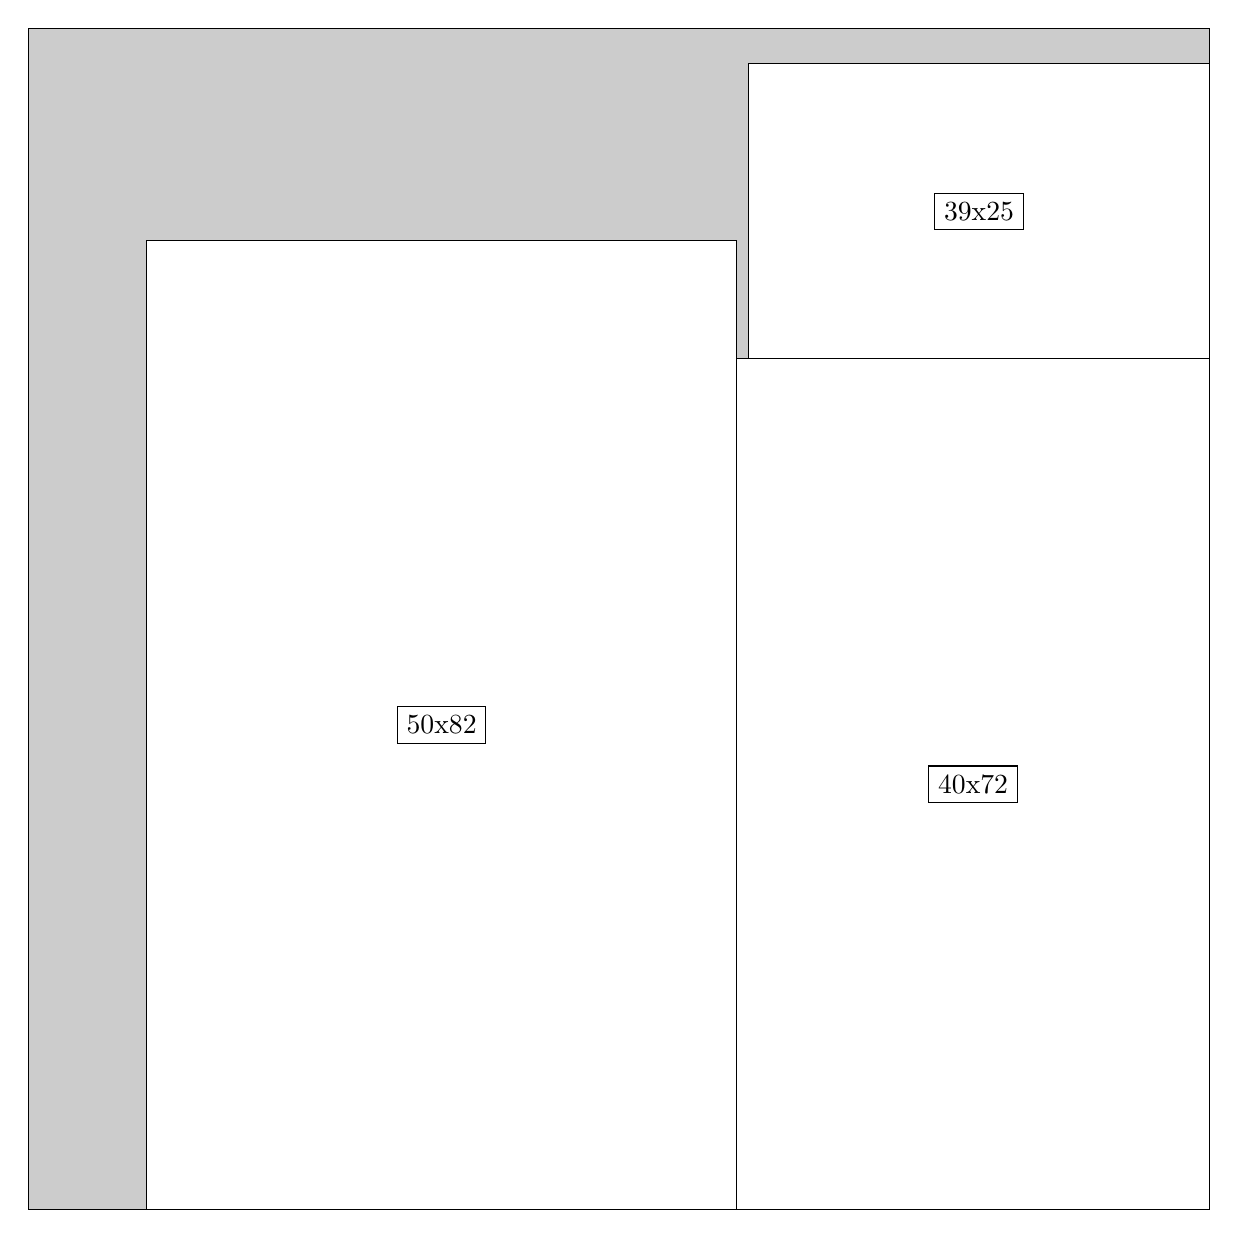
\begin{tikzpicture}[shorten >=1pt,scale=1.0,every node/.style={scale=1.0},->]
\tikzstyle{vertex}=[circle,fill=black!25,minimum size=14pt,inner sep=0pt]
\filldraw[fill=gray!40!white, draw=black] (0,0) rectangle (15.0,15.0);
\foreach \name/\x/\y/\w/\h in {40x72/9.0/0.0/6.0/10.799999999999999,39x25/9.15/10.799999999999999/5.85/3.75,50x82/1.5/0.0/7.5/12.299999999999999}
\filldraw[fill=white!40!white, draw=black] (\x,\y) rectangle node[draw] (\name) {\name} ++(\w,\h);
\end{tikzpicture}


w =40 , h =72 , x =60 , y =0 , v =2880
\par
w =39 , h =25 , x =61 , y =72 , v =975
\par
w =50 , h =82 , x =10 , y =0 , v =4100
\par
\newpage


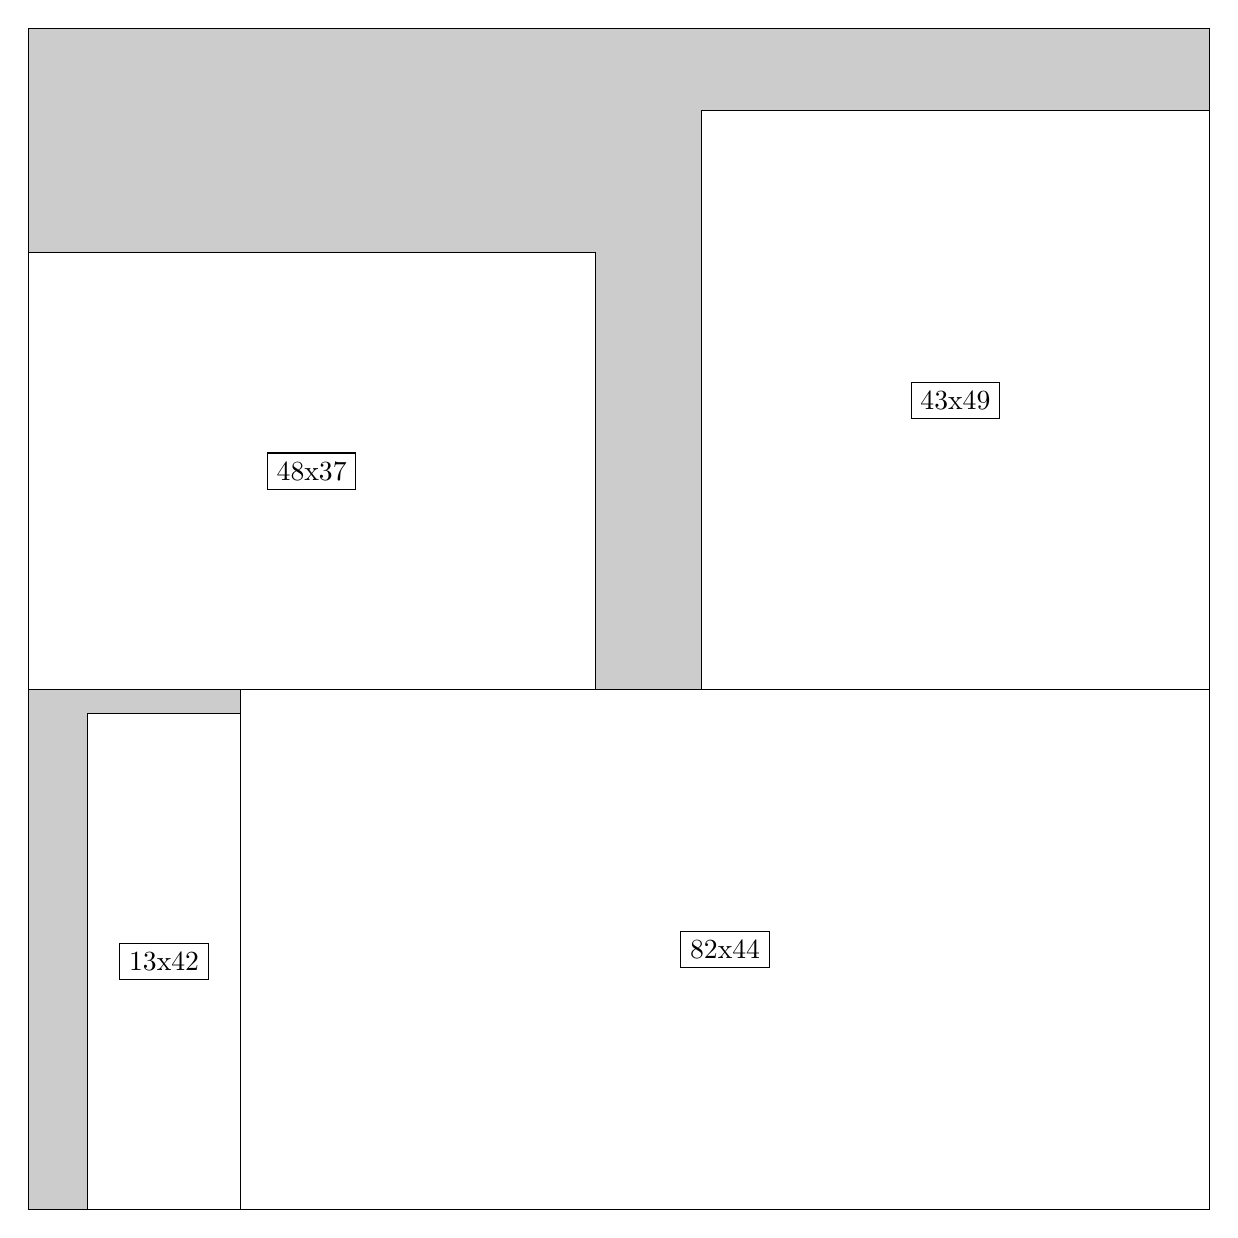
\begin{tikzpicture}[shorten >=1pt,scale=1.0,every node/.style={scale=1.0},->]
\tikzstyle{vertex}=[circle,fill=black!25,minimum size=14pt,inner sep=0pt]
\filldraw[fill=gray!40!white, draw=black] (0,0) rectangle (15.0,15.0);
\foreach \name/\x/\y/\w/\h in {82x44/2.6999999999999997/0.0/12.299999999999999/6.6,13x42/0.75/0.0/1.95/6.3,43x49/8.549999999999999/6.6/6.45/7.35,48x37/0.0/6.6/7.199999999999999/5.55}
\filldraw[fill=white!40!white, draw=black] (\x,\y) rectangle node[draw] (\name) {\name} ++(\w,\h);
\end{tikzpicture}


w =82 , h =44 , x =18 , y =0 , v =3608
\par
w =13 , h =42 , x =5 , y =0 , v =546
\par
w =43 , h =49 , x =57 , y =44 , v =2107
\par
w =48 , h =37 , x =0 , y =44 , v =1776
\par
\newpage


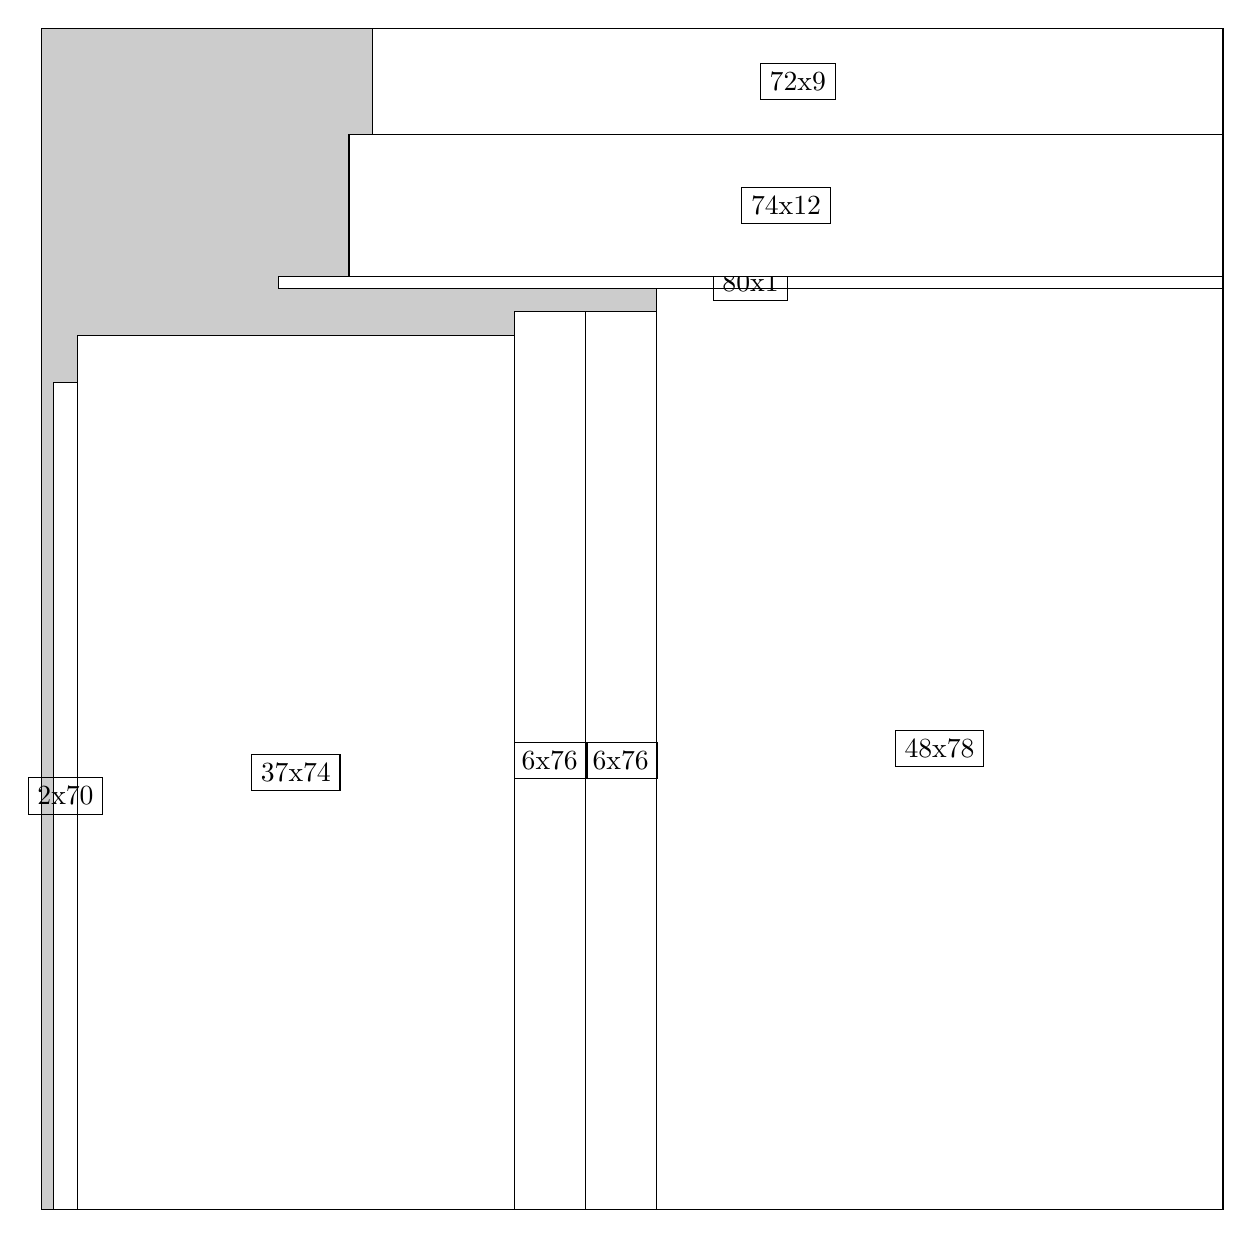
\begin{tikzpicture}[shorten >=1pt,scale=1.0,every node/.style={scale=1.0},->]
\tikzstyle{vertex}=[circle,fill=black!25,minimum size=14pt,inner sep=0pt]
\filldraw[fill=gray!40!white, draw=black] (0,0) rectangle (15.0,15.0);
\foreach \name/\x/\y/\w/\h in {48x78/7.8/0.0/7.199999999999999/11.7,6x76/6.8999999999999995/0.0/0.8999999999999999/11.4,6x76/6.0/0.0/0.8999999999999999/11.4,37x74/0.44999999999999996/0.0/5.55/11.1,2x70/0.15/0.0/0.3/10.5,80x1/3.0/11.7/12.0/0.15,74x12/3.9/11.85/11.1/1.7999999999999998,72x9/4.2/13.65/10.799999999999999/1.3499999999999999}
\filldraw[fill=white!40!white, draw=black] (\x,\y) rectangle node[draw] (\name) {\name} ++(\w,\h);
\end{tikzpicture}


w =48 , h =78 , x =52 , y =0 , v =3744
\par
w =6 , h =76 , x =46 , y =0 , v =456
\par
w =6 , h =76 , x =40 , y =0 , v =456
\par
w =37 , h =74 , x =3 , y =0 , v =2738
\par
w =2 , h =70 , x =1 , y =0 , v =140
\par
w =80 , h =1 , x =20 , y =78 , v =80
\par
w =74 , h =12 , x =26 , y =79 , v =888
\par
w =72 , h =9 , x =28 , y =91 , v =648
\par
\newpage


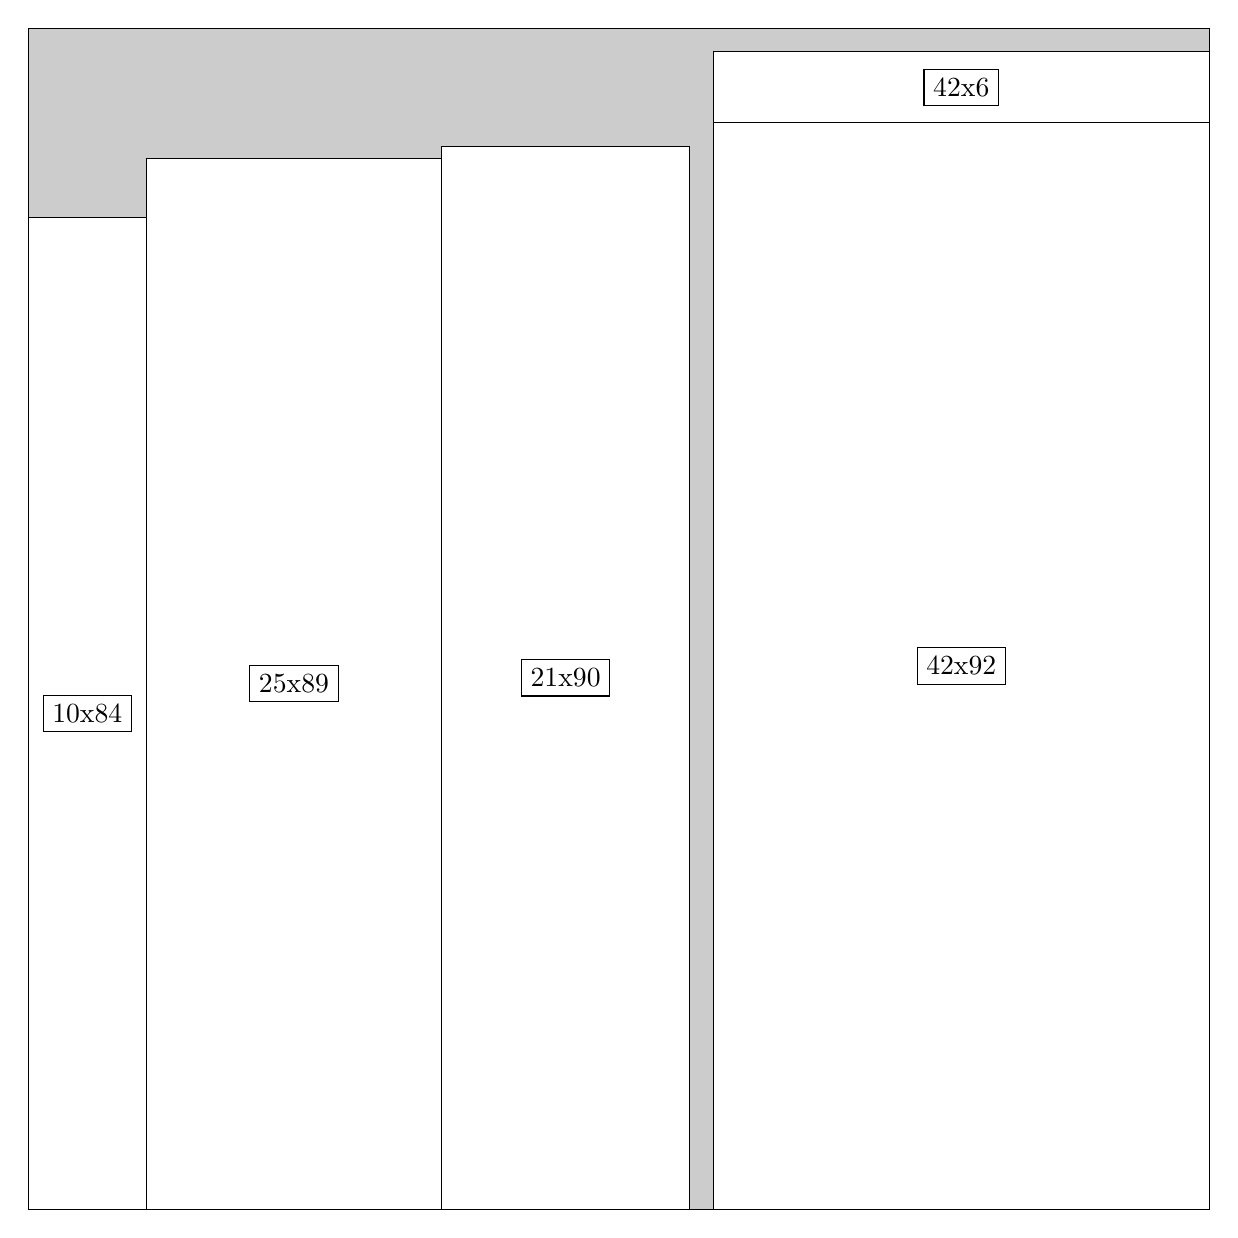
\begin{tikzpicture}[shorten >=1pt,scale=1.0,every node/.style={scale=1.0},->]
\tikzstyle{vertex}=[circle,fill=black!25,minimum size=14pt,inner sep=0pt]
\filldraw[fill=gray!40!white, draw=black] (0,0) rectangle (15.0,15.0);
\foreach \name/\x/\y/\w/\h in {42x92/8.7/0.0/6.3/13.799999999999999,42x6/8.7/13.799999999999999/6.3/0.8999999999999999,21x90/5.25/0.0/3.15/13.5,25x89/1.5/0.0/3.75/13.35,10x84/0.0/0.0/1.5/12.6}
\filldraw[fill=white!40!white, draw=black] (\x,\y) rectangle node[draw] (\name) {\name} ++(\w,\h);
\end{tikzpicture}


w =42 , h =92 , x =58 , y =0 , v =3864
\par
w =42 , h =6 , x =58 , y =92 , v =252
\par
w =21 , h =90 , x =35 , y =0 , v =1890
\par
w =25 , h =89 , x =10 , y =0 , v =2225
\par
w =10 , h =84 , x =0 , y =0 , v =840
\par
\newpage


\end{document}